\chapter{Statistika - setup a~základní postupy}
Představme si, že máme nějakou reálnou situaci a~chceme na~ní vytvořit statistický matematický model, který závisí na~jistých parametrech ($\t$). Narozdíl od~jiných předmětů ale máme k~dispozici výsledky měření z~navrženého experimentu a~zkoumáme jejich příčinu. Máme opět $\prostor$. $\Omega$ zde nazveme \textbf{populace}, $\omega\in\Omega$ nazveme \textbf{individuum}. 

Náhodná veličina $X:\Omega\to\R$ zde bude představovat \textbf{vlastnost} zkoumanou na~dané populaci $\Omega$ (např. počet špatných výrobků v~sérii). Tuto vlastnost zjišťujeme experimentálně, např. měřením, vážením apod. Víme také, že $X\sim\PP^X$ má jisté rozložení na~$\prostor$ dané např. pomocí  $\FF_X,f_X,p_X,...$, které ale neznáme a~chceme ho zjistit. 
\begin{define}
	n-tici nezávislých náhodných veličin $X_1,...,X_n$ stejně rozdělených s~distribuční funkcí $\FF$ nazýváme \textbf{náhodný výběr} z~rozdělení $\FF$. Konkrétní realizací $\X$ získáme vektor čísel $\textbf{x}=(x_1,...,x_n)$, který nazveme \textbf{realizace} náhodného výběru $X_1,...,X_n$, neboli naměřená data.
\end{define}
\begin{example}
	Příkladem je třeba $n$ opakování stejných experimentů, ve~kterých máme pokaždé stejné nastavení. Používáme tedy stejnou metodu měření. Dalším příkladem může být $n$ výrobků z~nějaké dodávky zboží, na~základě kterých určujeme celkový počet zmetků.
\end{example}

\begin{define} 
	Vybereme vektor individuí $\omega^{(n)}=(\omega_1,...,\omega_n)\in\Omega^n$ a~definujeme $$X_j\br{\omega^{(n)}}:=X(\omega_j),~\forall j\in\hat{n},$$ jako \textbf{pozorování} (v tomto tvaru máme skutečná data). Zavedeme dále $\Omega^{(n)}:=\Omega^n,$\newline$\Aa^{(n)}:=\sigma(\Aa^n)$, $\PP^{(n)}:=\bigotimes\limits_{1}^n \PP^X$ (součinová míra), tedy $$ \PP^{(n)}(A_1\times ...\times A_n)=\prod\limits_{j=1}^n \PP^X(A_j),~\forall A_j\in\Aa .$$
\\ \\
 Definujeme
	\textbf{realizaci} náhodného výběru $\X=(X_1,...,X_n)$ vztahem $$\textbf{x}=\X(\omega^{(n)}).$$
\end{define}

\begin{theorem}\label{iid}
	$\poslkon~iid~\PP^X$.
	\begin{proof} Pro~$\forall B\in\Bb$ a~$\forall j \in\widehat{n}$ platí, že 
		$$ \PP^{X_j}(B)=\PP^{(n)}\circ \inv{X_j}(B)=\PP^{(n)}\br{\underbrace{\{ X_j\in B \}}_{\Omega\times\Omega...\times\{ X\in B \}\times \Omega...}}=\PP(X\in B)=\PP^X(B). $$ Zbývá nám ještě dokázat nezávislost:
		$$ \PP^{(n)}\Br{\bigcap\limits_{j=1}^n\{ X_j\in B_j \}}=\PP^{(n)}\Br{\bigtimes\limits_{j=1}^n\{ X\in B_j \}}=\prod\limits_{j=1}^n\PP(X\in B_j)=\prod\limits_{j=1}^n\PP^{(n)}(X_j\in B_j), $$ protože $B_j$ jsou pokaždé na~jiné "pozici" v~kartézském součinu $\Omega\times...\times\{ X\in B_j \}\times...\times\Omega$.
	\end{proof}
\end{theorem}
\begin{define}
		\textbf{Statistika} je libovolná funkce náhodného výběru $X_1,...,X_n$, jejíž funkční předpis nezávisí na~parametrech příslušného rozdělení.
		\\ \\
	Příkladem statistiky může být \textbf{výběrový průměr} (sample mean)$$\Oxn=\frac{1}{n}\sumjn X_j,$$ případně \textbf{geometrický průměr}
	$$ \Oxn^G=\sqrt[n]{X_1X_2...X_n}, $$\textbf{výběrový rozptyl}
	$$ \hsn=\frac{1}{n}\sumjn(X_j-\Oxn)^2\text{ \quad nebo\quad  }s_n^2=\frac{1}{n-1}\sumjn (X_j-\Oxn)^2,$$ kde $\widehat{\sigma}_n$ nebo případně $s_n$ je \textbf{výběrová směrodatná odchylka}. Dále uveďme \textbf{$r$-tý výběrový obecný a~centrální moment} (sample moments)
	$$m_r'=\frac{1}{n}\sumjn X_j^r,\qquad m_r=\frac{1}{n}\sumjn(X_j-\Oxn)^r,$$ 
	\textbf{medián}
	$$ \widehat{X}_{\frac{1}{2}} = \begin{cases}
	X_{(\frac{n+1}{2})} & n\text{ liché}, \\ \frac{1}{2}\br{X_{(\frac{n}{2})}+X_{(\frac{n}{2}+1)}} & n\text{ sudé},
	\end{cases} $$  kde $X_{(j)}$ značí $j$-tou zdola uspořádanou statistiku z~náhodného výběru $\br{X_{(1)}\leq...\leq X_{(n)}}$.
\end{define}



\section{Statistické bodové odhady}
Nechť $\t$ je parametr spojený s~rozdělením $\PP^X$, tzn. $\t=\t(\PP^X)$. Máme dvě možnosti. 
\begin{enumerate}[a)]
	\item $\t$ může být spojený s~$\PP^X$, např. $\t=\E X,\D X, \FF_X(t),...$, nebo
	\item $\t$ může být přímo parametr rozdělení $\PP_\t^X$.
\end{enumerate}
V obou případech ale požadujeme tzv. identifikovatelnost rodiny $\mathcal{P}=\{\PP^X\}$, resp.\\ $\mathcal{P}=\{\PP_\t^X:\t\in\Theta\}$, tzn., že každému parametru přísluší právě jedna pravděpodobnost $X$.
$$ \t_1\neq\t_2~\Rightarrow~\PP_1^X\neq\PP_2^X,\quad\text{resp.}\quad \t_1\neq \t_2 \Rightarrow P_{\t_1}^X\neq P_{\t_2}^X.$$
Opačná implikace často neplatí, třeba pro~danou střední hodnotu najdeme vícero různých rozdělení.
Předpokládáme, že $\t\in\Theta\subset \R^k$, kde $\Theta$ se~nazývá \textbf{parametrický prostor}. Dále máme $\tau(\t):\Theta\to\R^s$, kde $\tau$ je tzv. \textbf{parametrická funkce} (většinou nás ale zajímá např. jedna vybraná složka, tedy $s=1$). Odhadnout celé rozdělení se~nám většinou nepodaří (nebo to nepotřebujeme), proto hledáme odhad parametru $\t$. 

\begin{define}
	Libovolná (borelovsky) měřitelná funkce náhodného výběru $X_1,...,X_n$ (tedy statistika) \[
	\begin{split}
	\htn(\X)&:\Omega^n\to\R^k\text{ se~nazývá \textbf{odhadem} (estimator) }\t\in\Theta\subset\R^k. \\
	\widehat{T_n}(\X)&:\Omega^n\to\R^s\text{ se~nazývá \textbf{odhadem} (estimator) parametrické funkce }\tau(\t)\in\tau(\Theta)\subset\R^s.
	\end{split}
	\] 
\end{define}
\begin{remark}
	Tato definice nám však neříká, jak tuto statistiku volit. Aby však poskytovala námi žádané výsledky, je potřeba, aby splňovala některé vlastnosti.
\end{remark}

\section{Vlastnosti bodových odhadů}
\begin{define}
	$T_n(\X)$ nazýváme \textbf{nestranný odhad} $\tau(\t)$, pokud $$\E_\t T_n(\X)=\tau(\t),~\forall\t\in\Theta,~\forall n\in\N.$$  
	$T_n(\X)$ nazýváme \textbf{asymptoticky nestranný odhad} $\tau$, pokud $$\E_\t T_n(\X)\to\tau(\t),~\forall\t\in\Theta,$$
	kde $\E_\t$ značí střední hodnotu vzhledem k~rozdělení $\PP_\t^X$.
\end{define}
\begin{remark}
	Střední hodnotu tedy chápeme jako "průměrování" přes všechny možné výběry, které lze získat pod~rozdělením $\PP_\t^X$ při~daném fixním, ale libovolném $\t$.
\end{remark}

\begin{define}
	$T_n(\X)$ nazýváme \textbf{eficientní} (vydatný), pokud pro~$\forall\widetilde{T}_n,~\forall\t\in\Theta$ platí \[
	\begin{split}
	s=1:~&\E\Big[\br{T_n(\X)-\tau(\t)}^2\Big]\leq \E\Big[\br{\widetilde{T}_n(\X)-\tau(\t)}^2\Big], \\
	s>1:~&\E\Big[\nor{T_n(\X)-\tau(\t)}_{\epsilon}^2\Big]\leq \E\Big[\nor{\widetilde{T}_n(\X)-\tau(\t)}_{\epsilon}^2\Big].
	\end{split}
	\]  
	$\E(T_n-\tau)^2$ se~nazývá střední kvadratická chyba - MSE (\textit{mean squared error}) odhadu $T_n(\X)$. Tedy eficientní odhad má nejnižší možnou MSE. Pro~nestranné odhady $\br{\tau(\t)=\E T_n(\X)}$ tento vztah pro~$s=1$ přechází na~$\D T_n(\X)\leq \D \widetilde{T}_n(\X)$.
\end{define}

\begin{define}
	Máme-li $T_n^1,T_n^2:\Omega\to\R^1$ jako odhady $\tau(\t)$, pak definujeme \textbf{relativní eficienci} vztahem $$\RE=\frac{\E(T_n^1-\tau)^2}{\E(T_n^2-\tau)^2}\equal{\text{nestranný odhad}}\frac{\D T_n^1}{\D T_n^2}.$$
\end{define}


Zkusme nyní porovnat dvě statistiky tak, abychom určili, která z~nich je lepší. Pokud porovnáváme 2 nestranné statistiky, pak lepší (\textbf{vydatnější}) z~nich je ta s~menším rozptylem. Pokud však porovnáváme statistiky, které nejsou nestranné, pak nutně nemusí být lepší ta s~nižším rozptylem. Používáme k~tomu tedy právě definovanou \textbf{MSE} (střední kvadratickou odchylku, mean squared error) (viz obrázek \ref{fig:mse}) $$ \MSE(\hat{\t})=\E(\hat{\t}-\t)^2,\text{ kde $\hat{\t}$ je odhadem neznámého parametru $\t$.} $$
\begin{figure}[h]
	\centering
	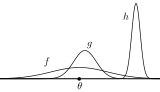
\includegraphics[width=0.4\linewidth]{Images/MSE}
	\caption{Ukázka toho, že statistika s~nejmenším rozptylem (h) nebo s~nejbližší střední hodnotou (f) nemusí být nutně ta nejvhodnější.}
	\label{fig:mse}
\end{figure}

\begin{define}
	$T_n(\X)$ se~nazývá \textbf{konzistentní} odhad $\tau$, pokud $$T_n(\X)\PSJ\tau(\t),\quad\forall\t\in\Theta$$ (pro $\Pto$ slabě konzistentní, pro~$\sj$ silně konzistentní).
\end{define}

\begin{theorem}[Kritérium konzistence]
	Odhad $T_n(\X)$ je slabě konzistentní $(T_n(\X)\Pto\tau(\t))$, pokud \begin{enumerate}
		\item $T_n(\X)$ je asymptoticky nestranný $(\E_\t T_n(\X)\to\tau(\t),$ pro~$\forall\t\in\Theta)$ a
		\item platí pro~něj, že $\D T_n(\X)\to0$.
	\end{enumerate}
\end{theorem}

\begin{example}
	Statistika je funkce náhodných veličin, a~proto se~taky chová jako náhodná veličina. Má proto taky své vlastní rozdělení a~například střední hodnota jejího rozdělení nám může poskytnout užitečné informace. Příkladem je zkoumání realizace exponenciálního rozdělení $\Exp(\frac{1}{2})$ (viz obr. \ref{fig:hist0}). Vezměme nyní statistiku "výběrový průměr" (výběrová střední hodnota). Na~obrázku \ref{fig:hist1} vidíme, že střední hodnota výběrového průměru odpovídá $\mu=\frac{1}{2}$, což je důsledek toho, že je statistika nestranná. Pro~vyšší $n$ jde zároveň její rozptyl k~nule. Tyto vlastnosti vyplývají z~centrální limitní věty, která říká, že výběrový průměr má přibližně normální rozdělení (pro data z~normálního rozdělení pak přímo normální rozdělení) dané vztahem
	$$ \Oxn\sim\AN\Br{\mu,\frac{\sigma^2}{n}}. $$
	%http://www.karlin.mff.cuni.cz/~hudecova/education/download/chem_predn/nahodny_vyber_tisk.pdf
	\begin{figure}[h]
		\centering
		\includegraphics[width=0.3\linewidth]{Images/histexp0}
		\caption{Hustota pravděpodobnosti rozdělení $\Exp(\frac{1}{2})$.}
		\label{fig:hist0}
	\end{figure}
	
	\begin{figure}[h]
		\centering
		\includegraphics[width=0.32\linewidth]{Images/histexp2}
		\includegraphics[width=0.32\linewidth]{Images/histexp50}
		\includegraphics[width=0.32\linewidth]{Images/histexp1000}
		\caption{Hustota pravděpodobnosti výběrového průměru pro~$n=2,~n=50$ a~$n=1000$. Vidíme tedy, že $\Oxn\sim\AN\Br{\mu,\frac{\sigma^2}{n}}$, kde $\mu=0.5$.}
		\label{fig:hist1}
	\end{figure}
\end{example}
\begin{define}
	$T_n(\X)$ se~nazývá \textbf{asymptoticky normálním} odhadem $\tau(\t)$ s~asymptotickou kovarianční maticí $\C(\t)$ (matice tvaru $s\times s$), pokud pro~$\forall\t\in\Theta$ $$ T_n(\X)\sim\AN_s\Br{\tau(\t),\frac{1}{n}\C(\t)}\text{, tzn. \quad } \sqrt{n}\br{T_n(\X)-\tau(\t)}\Dto \NN _s\br{\textbf{0},\C(\t)}\text{ (viz CLT)}. $$
	\\ \\
	Pro $s=1$ definice přechází na~$\sqrt{n}\br{T_n(\X)-\tau(\t)}\Dto \n{0,\sigma^2(\t)}$, kde $\sigma^2(\t)$ nazýváme asymptotický rozptyl odhadu $T_n(\X)$. 
\end{define}

\begin{define}
	Máme-li $T_n^1,T_n^2$ jako odhady $\tau(\t)$, které jsou oba $\AN$ odhady $\tau$ s~asymptotickými rozptyly $\sigma_1^2(\t)$ a~$\sigma_2^2(\t)$, pak definujeme \textbf{asymptotickou relativní eficienci} vztahem $\ARE=\frac{\sigma_1^2(\t)}{\sigma_2^2(\t)}$.
\end{define}

\begin{remark}
	\begin{itemize}
		\item Odtud nutně neplyne, že $\E\Br{\sqrt{n}\br{T_n(\X)-\tau(\t)}}\to 0 $ (tedy asymptotická nestrannost $T_n$), protože $\lim\limits_{n\to+\infty}\E T_n$ nemusí nutně existovat.
		\item Nemusí dokonce platit ani vztah $\D\Br{\sqrt{n}\br{T_n(\X)-\tau(\t)}}=\D\Br{\sqrt{n}\br{T_n(\X)}}\to\sigma^2(\t)$. (rovnítko vyplývá z~posunutí o~konstantu).
	\end{itemize}
\end{remark}

\begin{theorem}
	$T_n(\X)$ je asymptoticky normální $\AN\Br{\tau(\t),\frac{1}{n}\sigma^2(\t)}$. Pak $T_n(\X)\Pto\tau(\t),~\forall\t\in\Theta$. 
Tato slabá konzistence je řádu $o_p(n^{-\alpha}),~\alpha<\frac{1}{2}$, tzn., že $n^\alpha(T_n(\X)-\tau(\t))\Pto0,~\forall\alpha<\frac{1}{2}$. To vyplývá z~věty (MIP) $\Br{\text{Mějme }\posln,~X_n\sim\AN(\mu,\sigma_n^2)\text{ tak, že }\sigma_n\to 0.\text{ Pak }X_n\Pto \mu.}$.
\end{theorem}

\begin{theorem}[$\Delta$-metoda]\label{lamatko}
	Nechť $T_n(\X)\sim\AN\Br{\tau(\t),\frac{1}{n}\sigma^2(\t)}$ a~$g:\R^1\to\R^1$ spojitě diferencovatelnou v~$\tau(\t),~\forall\t\in\Theta$. Pak $$g\br{T_n(\X)}\sim\AN_1\left( g\br{\tau(\t)},\frac{\sigma^2(\t)}{n}\left[ g'\br{\tau(\t)} \right]^2 \right).$$
\end{theorem}
\begin{example}
	Například pokud $T_n(\X)=\Oxn,~g(t)=t^2,~g'(t)=2t$, pak$$ (\Oxn)^2\sim\AN(\mu^2,\frac{\sigma^2}{n}\cdot 4\mu^2). $$ 
	\begin{figure}[h]
		\centering
		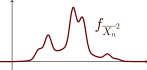
\includegraphics[width=0.3\linewidth]{Images/fxn1} \raisebox{5.6ex}{$\stackrel{n\to+\infty}{\longrightarrow}$}
		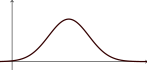
\includegraphics[width=0.3\linewidth]{Images/fxn2}
		\label{fig:fxn1}
	\end{figure}
\end{example}
\section{Výběrové charakteristiky a~jejich vlastnosti}
\begin{theorem}
	Mějme $X\in\LL_1$, resp. $\LL_2$, volme $\t=\t(\PP^X)=\E X=\mu$ a~označme \\$\sigma^2=\D X<+\infty~(\LL_2)$. Pak \textbf{sample mean} $$T_n(\X)=\Oxn=\frac{1}{n}\sumjn X_j$$ je nestranným, konzistentním a~$\AN\Br{\E X,\frac{1}{n}\sigma^2}$ odhadem $\t=\E X=\mu$.\begin{proof}Víme, že $X_1,...,X_n$ jsou $iid$ podle věty \ref{iid}. Pak
		\begin{enumerate} 
			\item $\E \Oxn=\mu,~\forall\mu$,
			\item $\Oxn\PSJ\E X$, což platí díky~ZVČ (Kolmogorov 2, kde požadujeme $\poslkon~iid ~\LL_1$),
		\end{enumerate}
	\end{proof}
\end{theorem}
\begin{remark}
	\begin{enumerate}
		\item CLT$_{L-L}$: $\Oxn\sim\AN\Br{\mu,\frac{\sigma^2}{n}}$ (zde požadujeme $\poslkon~iid~\LL_2$).
		\item 	$X$ zde značí vlastnost na~$\Omega$ a~$\X=(X_1,...,X_n)$ je náhodný výběr. Není to tedy realizace!
	\end{enumerate}

\end{remark}
\begin{theorem}
	$X\in\LL_2$, resp. $\LL_4$, volme $\t=\t(\PP^X)=\D X=\sigma^2$. Pak \textbf{výběrový rozptyl} $$T_n(\X)=\hsn=\frac{1}{n}\sumjn(X_j-\Oxn)^2\text{ \quad i\quad  }T_n(\X)=s_n^2=\frac{1}{n-1}\sumjn(X_j-\Oxn)^2$$ jsou oba asymptoticky nestranné, konzistentní a~$\AN\Br{\sigma^2,\frac{1}{n}(\mu_4-\sigma^4)}$ odhady $\sigma^2$, kde\\ $\mu_4=\E\left[ (X-\E X)^4 \right]$.
	V případě $T_n(\X)=s_n^2$ je $T_n(\X)$ navíc nestranný odhad $\sigma^2,~\forall n\in\N$.
	\begin{proof}Konzistence:
		$$ \hsn=\frac{1}{n}\sumjn(X_j-\Oxn)^2=\frac{1}{n}\sumjn X_j^2-\frac{2}{n}\sumjn X_j\Oxn+\Oxn^2=\underbrace{\frac{1}{n}\sumjn X_j^2}_{\overline{Y_n}\PSJ \E Y_1=\E X^2}-\underbrace{\Oxn^2}_{\to(\E X)^2}\PSJ \D X $$
		Nestrannost (pro $\hsn$ pouze asymptotická):
		\[
		\begin{split}
		\E\br{\hsn}&=\E \Br{\frac{1}{n}\sumjn X_j^2-(\Oxn)^2}=\E X^2-\E(\Oxn^2)=\E X^2-\frac{1}{n^2}\E\Br{\sumjn X_j^2-\sum\limits_{i\neq j}^nX_iX_j}=\\&=\E X^2-\frac{1}{n}\E X^2-\frac{1}{n^2}n(n-1)(\E X)^2=\frac{n-1}{n}\underbrace{\left[ \E (X^2)-(\E X)^2 \right]}_{=\D X=\sigma^2} =\frac{n-1}{n}\sigma^2\to \sigma^2,
		\end{split}
		\]
		$$ \E s_n^2=\frac{n}{n-1}\E \widehat{\sigma}_n^2=\sigma^2. $$ Asymptotická normalita $\hsn$ i~$s_n^2$ plyne z~rozkladu $\hsn=\frac{1}{n}\sumjn(X_j-\mu)^2-(\Oxn-\mu)^2$ a~ze~Slutskyho lemma.
	\end{proof}
\end{theorem}
\begin{remark}
	V případě dat \ref{fig:hist0}, kde $\sigma^2=0.25$ je situace zachycena na~obrázku \ref{fig:hist2}.
	
\end{remark}
\begin{dusl}
	Mějme $X\in\LL_2$.	Potom pro~tzv. \textbf{t-statistiku} platí, že $$t_n=t_n(\X)=\frac{\sqrt{n}(\oxn-\mu)}{s_n}\Dto\NN(0,1).$$\begin{proof}
		Z CLT$_{L-L}$	$$ \sqrt{n}(\Oxn-\mu)\Dto\NN(0,\sigma^2),\quad s_n\PSJ\sigma. $$
		Podíl tedy konverguje v~distribuci (Slutsky),
		$$ \frac{\sqrt{n}(\Oxn-\mu)}{s_n}\Dto\frac{\NN(0,\sigma^2)}{\sigma}=\NN(0,1). $$
	\end{proof}	\begin{figure}[h]
		\centering
		\includegraphics[width=0.32\linewidth]{Images/histexp_var2}
		\includegraphics[width=0.32\linewidth]{Images/histexp_var100}
		\includegraphics[width=0.32\linewidth]{Images/histexp_var1000}
		\caption{Histogram výběrového rozptylu realizace \ref{fig:hist0} (10000000 rozptylů) pro~$n=2$, $n=100$ a~$n=1000$. }
		\label{fig:hist2}
	\end{figure}
\end{dusl}

\begin{theorem}[Chinčin]
	Mějme $X\in\LL_r$, resp. $X\in\LL_{2r},~r\geq 1$, volíme $$\t_1=\t_1(\PP^X)=\E(X^r)=\mu'_r,\qquad\t_2=\E(X-\E X)^r=\mu_r.$$ Pak $r$-tý výběrový moment
	$$m_r'=m_r'(\X)=\frac{1}{n}\sumjn X_j^k$$
	je nestranným, konzistentním a~$\AN$ odhadem $\t_1=\mu'_1$ a~ $$m_r=m_r(\X)=\frac{1}{n}\sumjn(X_j-\oxn)^r$$ je konzistentním odhadem $\mu_r$.
\end{theorem}

\begin{theorem}Speciálně nyní mějme $(X_j)_{j=1}^{n,+\infty}~iid~\n{\mu,\sigma^2}$. Pak \begin{enumerate}[a)]
		\item $\Oxn\sim\n{\mu,\frac{\sigma^2}{n}},~\forall n\in\N$. Dále potom $\E \Oxn=\mu$, $\D\Oxn=\sigma^2$, $\frac{\sqrt{n}(\oxn-\mu)}{\sigma}\sim\n{0,1}$,
		\item $\hsn=\frac{1}{n}\sumjn(X_j-\Oxn)^2\quad \stackrel{\NN}{\Rightarrow}\quad \frac{n\hsn}{\sigma^2}\sim\chi^2(n-1),~\forall n\in\N$ (Pearsonovo rozdělení).\newline
		$s_n^2=\frac{1}{n-1}\sumjn(X_j-\Oxn)^2\quad \stackrel{\NN}{\Rightarrow}\quad \frac{(n-1) s_n^2}{\sigma^2}\sim\chi^2(n-1),~\forall n\in\N$. Dále platí
		\[
		\begin{split}
		\D(\hsn)&=\frac{\sigma^4}{n^2}2(n-1)=\frac{n-1}{n^2}(2\sigma^4)\to 0, \\
		\D(s_n^2)&=\D\left( \frac{\sigma}{n-1}\chi^2(n-1) \right)=\frac{\sigma^4}{(n-1)^2}2(n-1)=\frac{2\sigma^4}{n-1}\to0, \\
		\D(s_n^2)&>\D(\hsn).
		\end{split}
		\]
		\item $\Oxn$ a~$s_n^2$ jsou nezávislé a~platí 
		$$ \frac{\sqrt{n}(\oxn-\mu)}{s_n}=\frac{\frac{\sqrt{n}(\oxn-\mu)}{\sigma}}{\frac{s_n}{\sigma}}\sim\frac{\n{0,1}}{\sqrt{\frac{\chi^2(n-1)}{n-1}}}\sim t(n-1),~\forall n\in\N \text{ (Studentovo rozdělení).}$$
		\item Pokud jsou $X,Y$ na~$\prostor$ nezávislé, pak pro
		\begin{align*}
		&X_1,...,X_n~iid~\n{\mu_1,\sigma_1^2}\text{, ze~kterých známe } \Oxn,s_{1,n}^2, \\
		&Y_1,...,Y_m~iid~\n{\mu_2,\sigma_2^2}\text{, ze~kterých známe }  \overbar{\rule{0ex}{1.8ex}Y_m},s_{2,m}^2,
		\end{align*} platí, že 
		$$ \frac{s_{1,n}^2(n-1)}{\sigma_1^2}\sim\chi^2(n-1),\qquad \frac{s_{2,m}^2(m-1)}{\sigma_2^2}\sim\chi^2(m-1). $$
		Navíc lze ukázat, že $s_{1,n}^2$ a~$s_{2,m}^2$ jsou nezávislé.
	\end{enumerate}
\end{theorem}
\begin{dusl}
	$$ T_n(\X)=\frac{\frac{s_{1,n}^2}{\sigma_1^2}}{\frac{s_{2,m}^2}{\sigma_2^2}}=\frac{\frac{\chi^2(n-1)}{n-1}}{\frac{\chi^2(m-1)}{m-1}}\sim\FF(n-1,m-1)\quad\text{(Fisherovo rozdělení).} $$
\end{dusl}

\section{Výběrový kvantil (a jeho vlastnosti)}
\begin{define}
	Mějme náhodný výběr $(X_1,...,X_n)$. Pak $\left( X_{(1)},...,X_{(n)} \right)$ nazveme \textbf{uspořádaný náhodný výběr} (vzestupně). \textbf{Výběrový $\alpha$-kvantil} definujeme jako $\widehat{X}_{\alpha,n}=X_{([\alpha n]+1)} $, pro~$\alpha=\frac{1}{2}$ nazýváme $\widehat{X}_{\frac{1}{2}}$ \textbf{výběrovým mediánem}, který alternativně označujeme jako $\widehat{X}_\txt{med}$. \textbf{Výběrové rozpětí} pak definujeme jako $d=X_{(n)}-X_{(1)}$ a~\textbf{výběrové interkvartilové rozpětí} jako $$d_{\frac{1}{4}}=X_{\left( \left[\frac{3}{4}n\right]+1 \right)}-X_{\left( \left[\frac{1}{4}n\right]+1 \right)}.$$
\end{define}

\begin{remark}Připomeňme, že
	$\t=\t(\FF)=\inf\{ x:\FF(x)\geq \alpha \}\equal{\text{ozn}}x_\alpha$ je $\alpha$-kvantil rozdělení $\FF$. Pro~$\FF$ rostoucí a~spojitou potom $\FF(x_\alpha)=\alpha,~\alpha\in(0,1)$. Výběrový kvantil $\widehat{X}_{\alpha,n}$ je odhadem $x_\alpha$ a~zjednodušeně ho označujeme jako $\widehat{X}_\alpha$.
\end{remark}
\begin{example}~
		\begin{enumerate}
		\item Mějme data $\{1,2,3,4,5\}$, tedy $n=5$. Pak $\hat{x}_{1/2}=x_{[5/2]+1}=x_{(3)}=3=\overbar{\rule{0ex}{1.33ex}x_5}$.
		\item Nyní mějme $n=5$, ale tentokrát $\{1,2,3,4,500\}$. Pak $\hat{x}_{1/2}=3$ (je robustní), ale $\overbar{\rule{0ex}{1.33ex}x_5}=102$ (není robustní, tedy neodolá jedné, či několika větším výchylkám nebo chybám (\textit{outliers}) v~datech).
	\end{enumerate}
\end{example}
\begin{theorem}
	Mějme $X_1,...,X_n~iid~\FF,~\t=x_\alpha,~\alpha\in(0,1)$. Nechť $x_\alpha$ je jednoznačně určeno rovnicí $\FF(x_\alpha)=\alpha$ a~existuje $\FF'(x_\alpha)>0$. Pak $$\widehat{X}_\alpha\sim\AN\Br{x_\alpha,\frac{\alpha(1-\alpha)}{n[\FF'(x_\alpha)]^2}}.$$
	\begin{proof} Dokážeme, že platí vztah
		$Y_n:=\sqrt{n}(\widehat{X}_\alpha-x_\alpha)\Dto\n{0,\frac{\alpha(1-\alpha)}{[\FF'(x_\alpha)]^2}}$. Máme
		\[
		\begin{split}
		\FF_{Y_n}(t)=\PP(Y_n\leq t)=\PP\br{\sqrt{n}(\widehat{X}_\alpha-x_\alpha)\leq t}=\PP\br{\widehat{X}_\alpha\leq x_\alpha+\frac{t}{\sqrt{n}}}=\circledast
		\end{split}
		\]
		Nyní označme $S_n=\#\Big\{ j\in\hat{n}:\underbrace{X_j\leq x_\alpha+\frac{t}{\sqrt{n}}}_{A,~iid~\FF} \Big\}$. Pak $S_n\sim\mathrm{Bi}(n,p_n)$, kde 
		$$p_n=\PP(A)=\PP(X_j\leq x_\alpha+\frac{t}{\sqrt{n}})=\FF(x_\alpha+\frac{t}{\sqrt{n}}).$$  Dále si připomeneme vztah $\widehat{X}_\alpha=X_{([\alpha n]+1)}$, ve~kterém označíme $m=[\alpha n]+1$.\newline
		$$ \circledast = \PP(S_n\geq m)=1-\PP(S_n\leq m-1)\text{, který se~dá převést na~}1-\Phi_\mathcal{N}(...)\text{, protože }$$
		$$S_n\stackrel{\text{CLT}}{\sim}\AN\big(np_n,np_n(1-p_n)\big).$$
	\end{proof}
\end{theorem}
\begin{dusl}
	Z $\AN$ plyne, že $\widehat{X}_\alpha\Pto x_\alpha$ řádu $o_p(n^{-\beta}),~\beta<\frac{1}{2}$.
\end{dusl}

\section{Neparametrické (empirické) odhady distribucí}
\begin{define}
	Mějme $X_1,...,X_n~iid~\FF$, označme pro~dané $t\in\R$  charakteristickou funkci na~intervalu $(-\infty,t]$ jako $\Identita{(-\infty,t]}$. Pak \textbf{empirickou distribuční funkci} (EDF) $\FF_n$ definujeme vztahem $$\FF_n(t)=\FF_n(t,\X)=\frac{1}{n}\sumjn \Identita{(-\infty,t]}(X_j),\quad \forall t\in\R.$$ Pro~$t$ fixní můžeme psát $\FF_n(t,\X)=T_n(\X)$.
	\begin{center}
		\begin{tikzpicture}
		\node[inner sep=0pt] (pic) at (0,0)
		{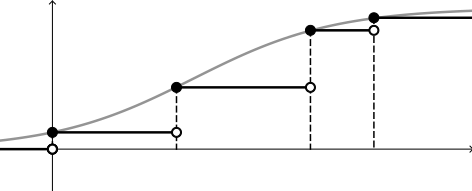
\includegraphics[width=6cm]{Images/mira}};
		\draw [color=black](-2.3,-0.75) node[anchor=north west] {$x_1$};
		\draw [color=black](-1,-0.75) node[anchor=north west] {$x_2$};
		\draw [color=black](0.7,-0.75) node[anchor=north west] {$x_3$};
		\draw [color=black](1.5,-0.75) node[anchor=north west] {$x_4$};
		\draw [color=black](-3.1,-0.85) node[anchor=north west] {$...$};
		\draw [color=black](2.2,-0.85) node[anchor=north west] {$...$};
		\end{tikzpicture}
	\end{center}
\end{define}

\begin{theorem}[ZVMS]
	Mějme $X_1,...,X_n~iid~\FF$. Pak pro~$\forall t\in\R$ fixní platí, že $\FF_n(t)$ je nestranným, konzistentním a~$\AN$ odhadem $\t=F(t)$, tzn.\begin{enumerate}
		\item $\E \FF_n(t)=\FF(t),~\forall n$,
		\item $\FF_n(t)\PSJ \FF(t),~\forall t\in\R$,
		\item $\FF_n(t)\sim\AN\left( \FF(t),\frac{1}{n}\FF(t)\br{1-\FF(t)} \right)$. 
\end{enumerate}	
	Navíc dokonce platí, že\begin{enumerate}
		\item $\sup\limits_{t\in\R}\abs{\FF_n(t)-\FF(t)}\sj 0$, (Glivenko-Cantelliho lemma),
		\item $\p{\sup\limits_{t}\abs{\FF_n(t)-\FF(t)}>\epsilon}\leq 8(n+1)\e{-\frac{n\epsilon^2}{32}},~\forall n,~\forall\epsilon>0$, (Glivenko-Cantelli),
		\item $\p{\sup\limits_{t}\abs{\FF_n(t)-\FF(t)}>\epsilon}\leq 2\e{-2n\epsilon^2},~\forall n,~\forall\epsilon>0$ (Massart, 1990).
	\end{enumerate}
	\begin{proof}
	Pro důkaz volme fixní libovolné $t$ a~označme $\Identita{(-\infty,t]}(X_j)=Y_j^t$. Pak
			 $Y_j^t=\begin{cases}
			1, & X_j\leq t, \\ 0, & \text{jinak,}
			\end{cases}$ přičemž spočteme
		$$ \PP(Y_j^t=1)=\PP(X_j\leq t)\equal{X_j~iid}P(X\leq t)=\FF(t),\quad\PP(Y_j^t=0)=1-\FF(t), $$ což nám poskytuje rozdělení $ Y_j^t\sim\A(p=\FF(t))$ - alternativní (Bernoulliho) rozdělení. $(Y_j^t)_{j=1}^n$ jsou nezávislé, protože $X_j~iid$.
		 Dále víme, že $n\FF_n(t)=\sumjn Y_j^t\sim \mathrm{Bi}\br{n,p=\FF(t)}$. Z~vlastností binomického rozdělení potom vyplývá, že 
			\begin{enumerate}[a)]
				\item $\E \FF_n(t)=\frac{1}{n}\E\big[ \mathrm{Bi}\br{n,p=\FF(t)} \big]=\FF(t)=\t,~\forall t$,
				\item $\frac{1}{n}\sumjn Y_j^t =\overbar{Y_n^t}\PSJ  \E Y_j^t=\E Y_1^t=\FF(t)=\t$\quad (ZVČ),
				\item $\FF_n(t)=\frac{1}{n}\sumjn Y_j^t =\overbar{Y_n^t}\sim\AN\Br{\FF(t),\frac{1}{n}\FF(t)\br{1-\FF(t)}}\quad\Br{\text{ CLT pro~}(Y_j^t)_{j=1}^n~iid~\LL_2\br{\mathrm{A}(p)}}$.
			\end{enumerate}
	\end{proof}
\end{theorem}

\begin{define}
	Mějme $\t=\t(\FF)$ (funkcionál na~prostoru distribučních funkcí). Pak $$T_n(\X)=\t(\underbrace{\FF_n}_{\to \FF})$$ se~nazývá \textbf{statistický funkcionál}.
\end{define}
\begin{example}
	\[
	\begin{split}
	\t(\FF)=\E X\quad &\Rightarrow\quad T_n(\X)=\t(\FF_n)=\int x\d\FF_n=\sumjn x_j\cdot\PP_n(X=x_j)=\sumjn x_j\cdot \frac{1}{n}=\Oxn, \\
	\t(\FF)=\D X\quad &\Rightarrow\quad  T_n(\X)=\t(\FF_n)=\int x^2\d\FF_n-\left( \int x\d\FF_n \right)^2=\frac{1}{n}\sumjn x_j^2-\Oxn^2=\hsn, \\
	\t(\FF)=x_{\alpha} \quad&\Rightarrow\quad T_n(\X)=\t(\FF_n)=\inf\{ x:\FF_n(x)\geq\alpha \}=\widehat{x}_\alpha,\text{ kde $x_\alpha$ je $\alpha$-kvantil $X$}.
	\end{split}
	\]
\end{example}
\begin{define}[Histogram]
	Mějme $X\sim f,~\supp f=[a,b]$, resp. zde BÚNO $[0,1]$. Zavedeme dělení intervalu $[0,1]$
	$$ B_1=\Big[0,\frac{1}{m}\Big),~B_2=\Big[\frac{1}{m},\frac{2}{m}\Big),...,~B_m=\Big[\frac{m-1}{m},1\Big] $$
	 a~označíme dále $h=\frac{1}{m}=\lambda(B_j)$, $Y_j=\#\{ i: X_i\in B_j \}_{i=1}^n$, $\widehat{p_j}=\frac{Y_j}{n}$ jako odhad $p_j=\int\limits_{B_j}f(x)\d x$. Pak \textbf{histogramový odhad hustoty pravděpodobnosti} definujeme vztahem
	$$ \widehat{f}_n^\txt{~H}(t)=\sm{j=1}{m}\frac{\widehat{p_j}}{h}\Identita{B_j}(t)=\frac{1}{nh}\sm{j=1}{m}Y_j\Identita{B_j}(t)=\frac{1}{nh}\sm{i=1}{n}\mathcal{I}{\{X_i\in B_j\}},\quad\forall t\in B_j. $$
\end{define}
\begin{theorem}[IMSE]
	Pro $\widehat{f}_n^\txt{~H}(t)$ předpokládejme, že $f'$ je absolutně spojitá a~platí, že\\ $\int\limits_{\R}\br{f'(u)}^2\d u<+\infty$. Potom
	$$ R(\widehat{f}_n^\txt{~H},f)=\frac{h^2}{12}\int\limits_{0}^1\br{f'(x)}^2\d x+\frac{1}{nh}+o(h^2)+o\Br{\frac{1}{n}}, $$
	což při~volbě $h_n=O\br{n^{-1/3}}$ vede na~řád integrované střední kvadratické chyby (\textit{Integrated Mean Square Error})
	$$ \txt{IMSE}=R(\widehat{f}_n^\txt{~H},f)=\int\limits_{0}^1\EE{\widehat{f}_n^\txt{~H}(t)-f(t)}^2\d t=O\br{n^{-2/3}}. $$
\end{theorem}
\begin{define}
	Mějme jádro $K(x)$ takové, že $K(x)\geq0,~\int\limits_{\R}K(x)\d x=1,~\int\limits_{\R}xK(x)\d x=0,~\sigma_K^2=\int\limits_{\R}x^2K(x)\d x>0$. Označíme $h\in\R^+$ jako tzv. \textbf{šířku okna} (\textit{bin width}), neboli vyhlazovací parametr (\textit{smoothing parameter}). Pak definujeme \textbf{jádrový odhad hustoty} vztahem
	$$ \widehat{f}_n^\txt{~K}(t):=\frac{1}{n}\sm{i=1}{n}\frac{1}{h}K\Br{\frac{t-X_i}{h}},\quad\forall t\in\R. $$
\end{define}
\begin{remark}
	Příklady takových používaných jader mohou být: \begin{enumerate}
		\item $K(x)=\frac{1}{2}\Identita{[-1,1]}(x)$ (boxcar),
		\item $K(x)=\frac{1}{\sqrt{2\pi}}\e{-\frac{x^2}{2}}$ (Gaussovo),
		\item $K(x)=\frac{3}{4}(1-x^2)\Identita{[-1,1]}(x)$ (Epanechnikovo) apod.
	\end{enumerate}
\end{remark}
\begin{remark}
Podobný výsledek řádu IMSE lze ukázat pro~jádrový odhad $\widehat{f}_n^\txt{~K}(t)$. Při~volbě $h_n=O\br{n^{-1/5}}$ lze dosáhnout pro~$\widehat{f}_n^\txt{~K}(t)$ řád IMSE$=O\br{n^{-4/5}}$.
\end{remark}